% This file was created with tikzplotlib v0.10.1.
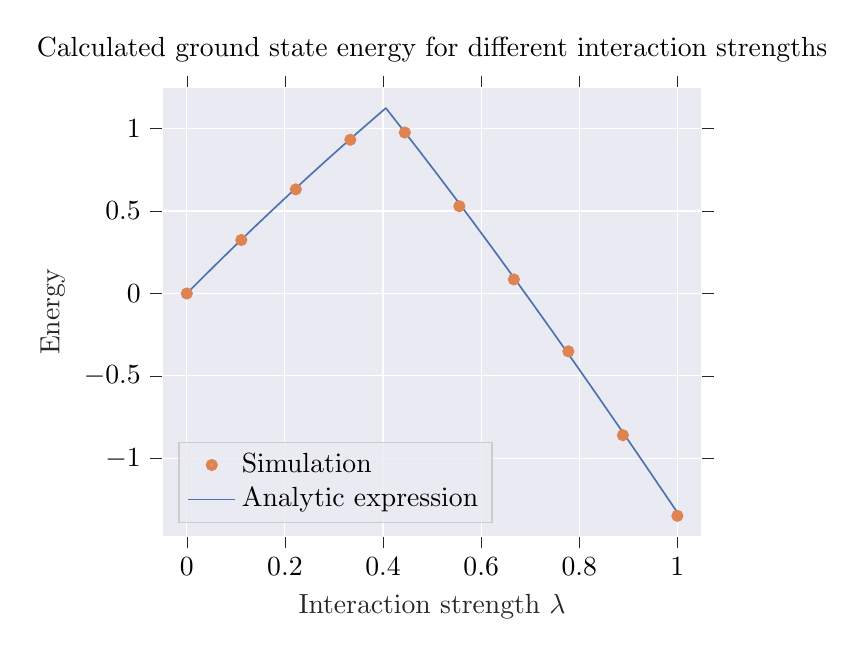
\begin{tikzpicture}

\definecolor{darkslategray38}{RGB}{38,38,38}
\definecolor{lavender234234242}{RGB}{234,234,242}
\definecolor{lightgray204}{RGB}{204,204,204}
\definecolor{peru22113282}{RGB}{221,132,82}
\definecolor{steelblue76114176}{RGB}{76,114,176}

\begin{axis}[
axis background/.style={fill=lavender234234242},
axis line style={white},
legend cell align={left},
legend style={
  fill opacity=0.8,
  draw opacity=1,
  text opacity=1,
  at={(0.03,0.03)},
  anchor=south west,
  draw=lightgray204,
  fill=lavender234234242
},
mark options={mark size=1.4pt, line width=1.5pt},
minor xtick={},
minor ytick={},
tick align=outside,
title style={align=center},
title={Calculated ground state energy for different interaction strengths},
x grid style={white},
xlabel=\textcolor{darkslategray38}{Interaction strength \(\displaystyle \lambda\)},
xmajorgrids,
xmajorticks=false,
xmajorticks=true,
xmin=-0.05, xmax=1.05,
xtick style={color=darkslategray38},
xtick={-0.2,0,0.2,0.4,0.6,0.8,1,1.2},
y grid style={white},
ylabel=\textcolor{darkslategray38}{Energy},
ymajorgrids,
ymajorticks=false,
ymajorticks=true,
ymin=-1.47185236333669, ymax=1.24703439569554,
ytick style={color=darkslategray38},
ytick={-1.5,-1,-0.5,0,0.5,1,1.5}
]
\addplot [draw=peru22113282, fill=peru22113282, mark=*, only marks]
table{%
x  y
0 0
0.111111111111111 0.324459499782986
0.222222222222222 0.631581624348958
0.333333333333333 0.932332356770833
0.444444444444444 0.976348876953125
0.555555555555556 0.529446072048611
0.666666666666667 0.0853780110677085
0.777777777777778 -0.350857204861111
0.888888888888889 -0.859446207682291
1 -1.3482666015625
};
\addlegendentry{Simulation}
\addplot [semithick, steelblue76114176]
table {%
0 0
0.0360000133514404 0.107259511947632
0.0709999799728394 0.210120677947998
0.105999946594238 0.311585307121277
0.141000032424927 0.411657810211182
0.175999999046326 0.5103440284729
0.210999965667725 0.607651233673096
0.246000051498413 0.703588604927063
0.281000018119812 0.798166513442993
0.315999984741211 0.89139711856842
0.351000070571899 0.983293533325195
0.386000037193298 1.07387053966522
0.404999971389771 1.12249386310577
0.406000018119812 1.12344861030579
0.440000057220459 0.994959950447083
0.473999977111816 0.86469841003418
0.509000062942505 0.728824377059937
0.545000076293945 0.587259888648987
0.58299994468689 0.435928583145142
0.621999979019165 0.278679251670837
0.661999940872192 0.115463733673096
0.703000068664551 -0.0537568330764771
0.746000051498413 -0.233208179473877
0.789999961853027 -0.418803691864014
0.835999965667725 -0.614834070205688
0.884000062942505 -0.821423888206482
0.934000015258789 -1.03868114948273
0.986000061035156 -1.26669788360596
0.999000072479248 -1.32401323318481
};
\addlegendentry{Analytic expression}
\end{axis}

\end{tikzpicture}
